\chapter{The FPGA}
\label{cha:fpga}

\section{Opal Kelly}
\label{sec:fpga-opal}
The design is based on the XEM7310-A75 board. This is a USB 3.0 FPGA development board, featuring the Xilinx Artix-7 FPGA. The board is designed to boost productivity and testing capabilities of digital designs, providing ease of communication with its USB host interface. A Block Diagram of the device is provided in figure \ref{fig:xem-block-diagram}.
\begin{figure}
    \centering
    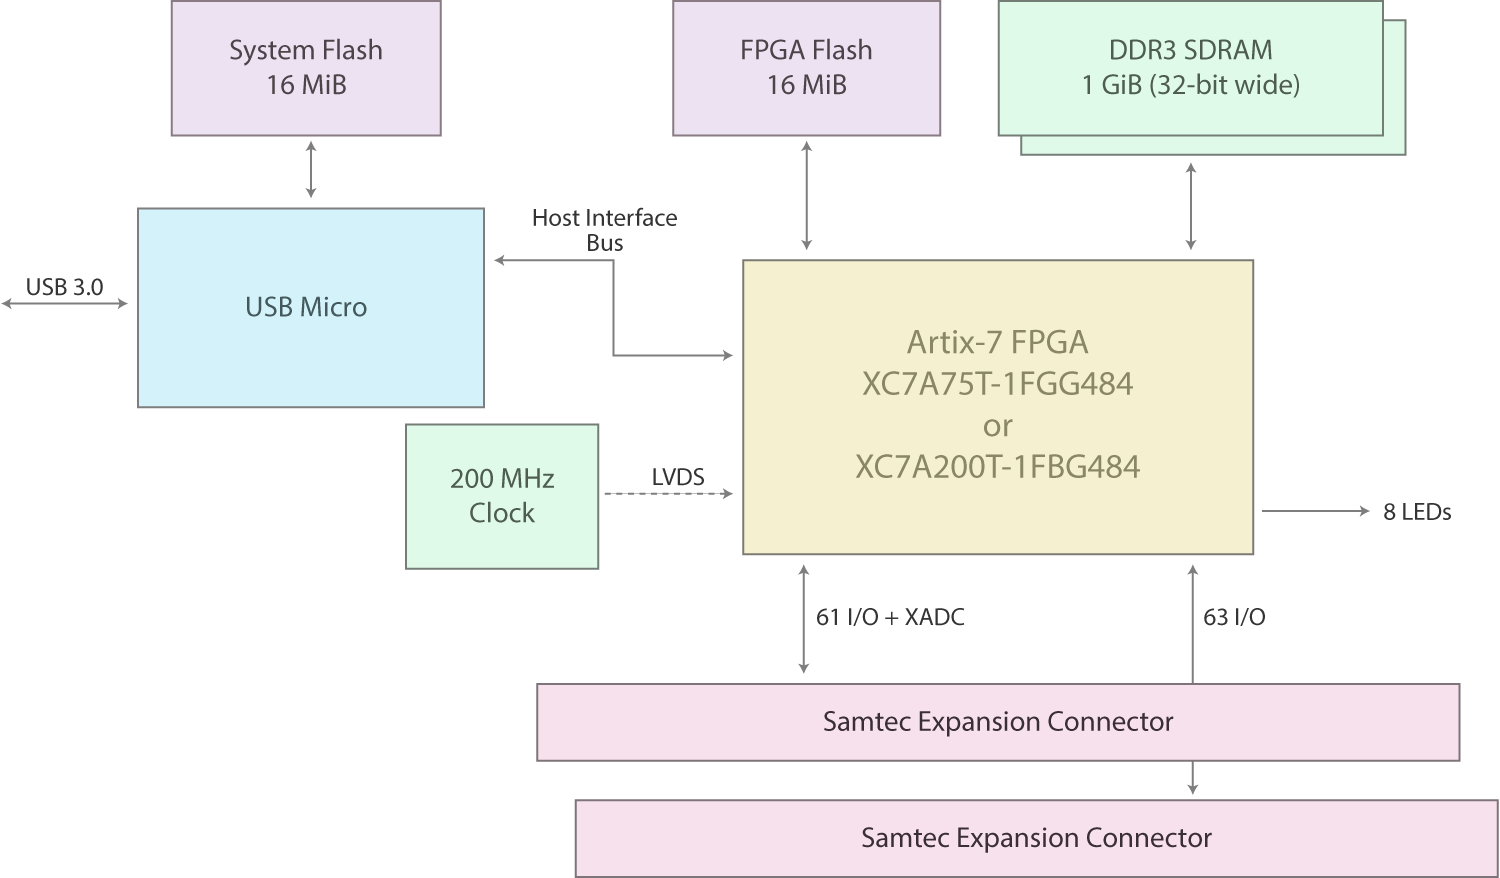
\includegraphics[width=0.5\linewidth]{lt_bachelor_disi_en//images/2XEM7310-BlockDiagram.png}
    \caption{XEM7310-A75 Block Diagram}
    \label{fig:xem-block-diagram}
\end{figure}

In particular, Opal Kelly provides an SDK (Software Development Kit) composed of several HDL modules, for example:
\begin{itemize}
    \item Virtual Trigger signals
    \item Two Pipes (in / out) for fast and easy communication between FPGA and a host pc
    \item Much more
\end{itemize}
This is a sketched overview:
\begin{figure}
    \centering
    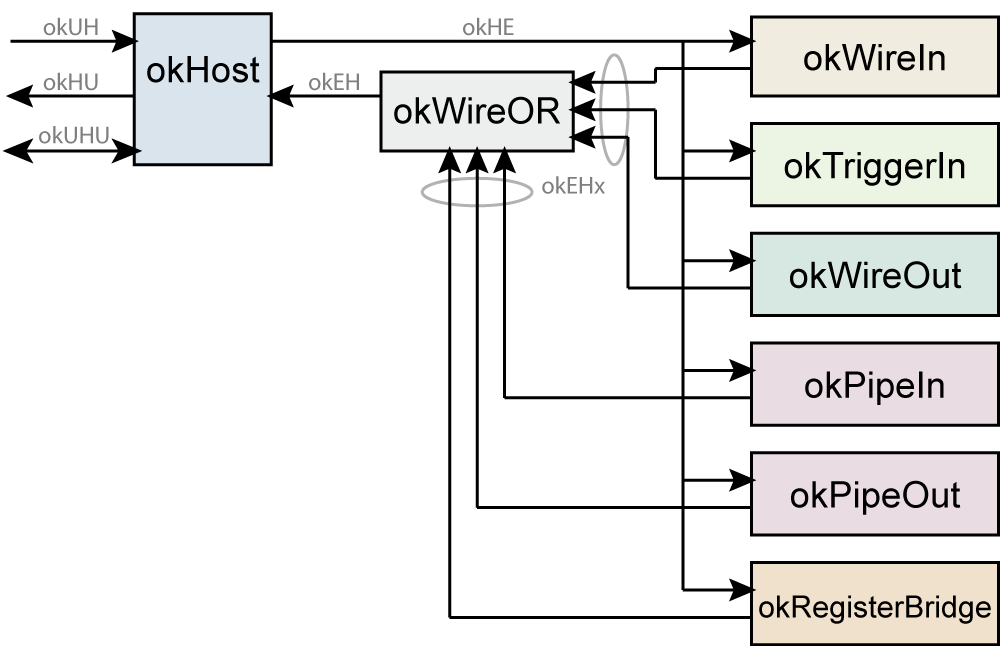
\includegraphics[width=0.5\linewidth]{lt_bachelor_disi_en//images/FrontPanelHDL-USB3.png}
    \caption{Opal Kelly HDL Overview}
    \label{fig:opal-kelly-hdl}
\end{figure}


\section{Xilinx Artix 7}
\label{sec:fpga-artix}
The specific FPGA mounted on the XEM7310-A75 is a Xilinx Artix-7. In particular, the model is the XC7A75T-1FGG, featuring:

\begin{table}[h!]
    \centering
    \begin{tabular}{|c|c|}
        \hline
        Slice Count & 11800 \\
        \hline
        D Flip Flops & 94400 \\
        \hline
        Distributed RAM & 892 Kib \\
        \hline
        Block RAM & 3,780 Kib \\
        \hline
        DSP Slices & 180\\
        \hline
        Clock Management Tiles & 6 \\
        \hline
    \end{tabular}
    \caption{Artix-7 Properties}
    \label{tab:artix-7-properties}
\end{table}

\section{Minimal Setup to Upload the bitstream file}
\label{sec:bitstream-setup}
The Opal Kelly full features in the SDK are going to be used later in the design process, but as a first step, I needed to set up a minimal environment to upload a bitstream file to the FPGA.

As mentioned before, Opal Kelly provides a host interface which can be used to ease the setup of the USB communication between a host computer and the Artix-7. In particular, they provide the \textit{FrontPanel SDK}, which is implemented for multiple programming languages to be used as a means of creating beautiful UIs in order to fetch and receive data from the FPGA.

My choice for the programming language was C++. Thus I set up a development environment on Microsoft Visual Studio, integrating the .NET framework, and in particular Windows Forms, in order to create a minimal UI to upload the bitstream onto the FPGA. This can be done easily via the FrontPanel SDK, as can be seen from the following function I implemented in \textit{myTools.h}:

\begin{lstlisting}[language={C++}, label={code:fpga-config}, caption={Function to Upload bitstream to FPGA (Made by my supervisor Alessandro Tontini)}]
okCFrontPanel* fpgaConfig(std::string bitfile_path){

	//Declare a new okCFrontPanel object
	okCFrontPanel *device = new okCFrontPanel();
	okCFrontPanel::ErrorCode error;

	//Load the FrontPanel DLL
	if (FALSE == okFrontPanelDLL_LoadLib(NULL)) {
		std::cout << "Could not load FrontPanel DLL\n";
		exit(-1);
	}else{
		std::cout << "FrontPanel DLL loaded successfully..\n";
	}
	
	/*Before any communication with the device can proceed, the device must be opened.
	  If no argument (string) is specified, the first appropriate device is opened, otherwise
	  specify the serial number by using GetDeviceListSerial*/
	
	if (device->OpenBySerial() != okCFrontPanel::NoError){
		std::cout << "An error has occured while trying to open the device. Error code is " << device->OpenBySerial() <<"\n";
		device -> ~okCFrontPanel();  //10/05/2018
		//return 0;
		return device;
	}else{
		std::cout << "Device opened successfully\n";
	}
		
	//Verify that the XEM7310 connected, otherwise exit
    if(device->GetBoardModel() != 43){
		std::cout << "Wrong XEM model. This program is targeted for XEM7310A75. ";
		std::cout << "Actual device: " << device -> GetBoardModel() << "\n";
    	device -> ~okCFrontPanel();
    	exit(-1);
	}
			
	//Configure the FPGA loading the specified bitfile
	std::cout << "Programming FPGA..\n";
	error = device -> ConfigureFPGA(bitfile_path);
	if(error == ok_ErrorCode:: ok_NoError){
		std::cout << "FPGA programmed succesfully.\nResult (error code): " << error << "\n";
	}else{
		std::cout << "An error has occured. Error code: " << error << "\n";
		device -> ~okCFrontPanel();
		exit(-1);
	}
		
	return device;
}
\end{lstlisting}



\section{Other Opal Kelly modules used in the design}


